\documentclass[11pt]{article}
\usepackage[T1]{fontenc}
\usepackage[french]{babel}
\usepackage{graphicx}
\usepackage[margin=2.5cm]{geometry}

\title{Bilan de masse du Glacier-Exemple, 2000-2024}
\author{Projet d'exemple d'Atelier}
\date{}

\begin{document}
\maketitle

\section{Introduction}
Le Glacier-Exemple est un glacier fictif. Ses valeurs servent seulement à
découvrir Atelier : compiler ce document, cliquer dans le PDF pour retrouver
la ligne source, demander une correction à l'agent.

\section{Résultats}
Le bilan de masse annuel est négatif presque chaque année depuis 2000
(figure~\ref{fig:bilan}). L'année 2022 est la plus déficitaire de la série.

\begin{figure}[h]
  \centering
  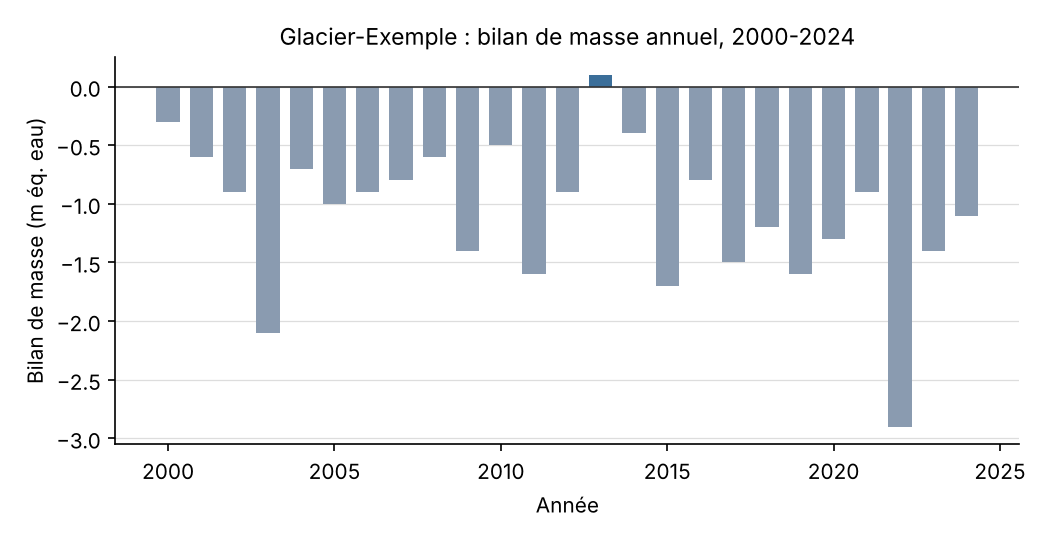
\includegraphics[width=\linewidth]{../figures/bilan_masse_annuel.png}
  \caption{Bilan de masse annuel, 2000-2024 (valeurs illustratives).}
  \label{fig:bilan}
\end{figure}

\section{Conclusion}
La perte de masse se poursuit sur toute la période.

\end{document}
